% 2012 年天津卷文科第 17 题：四棱锥 P-ABCD，底面 ABCD 为矩形，AD⊥PD。
% 来源 PDF：普通高考/2012/2012天津文.pdf，第 2 页（印面 778）第 1 栏。
% 重绘依据：原图为斜二测式透视：A、B 在前，C、D 在后，P 在上方偏左；
%   实线 PA、PB、PC、PD、AB、BC，虚线 AD、CD、AC。
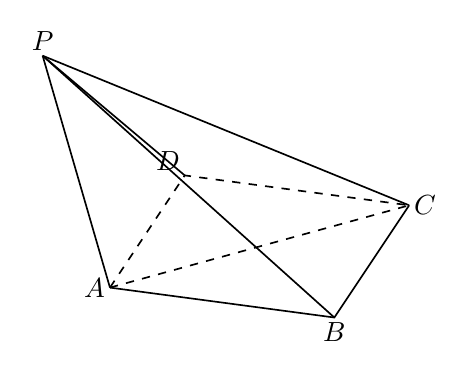
\begin{tikzpicture}[scale=0.95, semithick, every node/.style={inner sep=1.5pt}]
  \coordinate (A) at (0.4,0.5);
  \coordinate (B) at (3.4,0.1);
  \coordinate (C) at (4.4,1.6);
  \coordinate (D) at (1.4,2.0);
  \coordinate (P) at (-0.5,3.6);
  \draw (P) -- (A);
  \draw (P) -- (B);
  \draw (P) -- (C);
  \draw (P) -- (D);
  \draw (A) -- (B) -- (C);
  \draw[dashed] (A) -- (D) -- (C);
  \draw[dashed] (A) -- (C);
  \node[left] at (A) {$A$};
  \node[below] at (B) {$B$};
  \node[right] at (C) {$C$};
  \node[above left] at (D) {$D$};
  \node[above] at (P) {$P$};
\end{tikzpicture}
